\documentclass[12pt,a4paper,oneside]{report}
\usepackage{indentfirst}
\usepackage{times}
\setlength\parindent{1cm}
\renewcommand{\baselinestretch}{1.50}\normalsize
\usepackage{anysize}
\marginsize{1.25in}{.75in}{1in}{1in}
\usepackage{graphics}
\usepackage{graphicx}
\usepackage{epsfig}
\usepackage[fleqn]{amsmath}
\usepackage{amsfonts}
\usepackage{textcomp}
\usepackage{graphicx}
\usepackage{setspace}
\usepackage{fancyhdr}   
\usepackage{truncate}
\usepackage{nomencl} 
\usepackage{acronym}
\usepackage{array}
\usepackage{caption}\usepackage{subcaption}
\usepackage{subfig}
\usepackage[overload]{textcase}
\usepackage{listings}
\renewcommand{\nomname}{List of Abbreviations}
\usepackage{makeidx}
\makeindex
\makenomenclature
\newcommand{\quotes}[1]{``#1''}
\usepackage{titlesec}
\titleformat{\chapter}[display]
{\normalfont\Large\bfseries\centering}
{\chaptertitlename\ \thechapter}{15pt}{\LARGE}
\titleformat{\section}{\large\bfseries}{\thesection}{1em}{}
\titleformat{\subsection}{\normalsize\bfseries}{\thesubsection}{1em}{}
\renewcommand{\chaptermark}[1]{\markboth{ \emph{#1}}{}}

\printnomenclature[5em]
\pagestyle{fancy}
%\headheight 1pt
	\renewcommand{\footrulewidth}{1.2pt}
\renewcommand{\headrulewidth}{1.2pt}
\rhead{\scriptsize {\leftmark}}

\lhead{\small{College of Engineering, Cherthala \;\;\;\;\;\;\;\;\;\;\;\;\;\;\;\;\;\;}}
\rfoot{\thepage}
\cfoot{\empty}
\lfoot{\small{Department of Computer Science \& Engineering}}
\renewcommand{\figurename}{Fig.}
\begin{document}
\renewcommand\bibname{References}
\begin{titlepage}
\begin{center}
\large{\textbf{Design Report for}}\\
\begin{singlespace}
\LARGE{\textbf{Continuous Integration Pipeline Implementation \\ for
Tech11Software
}}\\
\end{singlespace}
\Large{\textit{Submitted By }}\\
\Large{\textit{\textbf{Aswin G Sugunan}     (13)}}\\
\Large{\textit{\textbf{Jefin Jacob}    (4)}}\\
\Large{\textit{\textbf{Nitin Suresh}   (23)}}\\
\Large{\textit{\textbf{Vishnu Bose}   (39)}}\\
\Large{\textit{\textbf{7th Semester}   }}\\

\Large{\textit{\textit{Under the guidance of}}}\\
\Large{\textit{\textbf{Mrs. Greeshma N Gopal }}}\\
\vspace{.05in}

\vspace{.05in}
\begin{figure}[h]
\begin{center}

\epsfig{width=1.5 in,file=logo.jpg}
\end{center}
\end{figure}
\begin{singlespace}
%\large{\textit{In partial fulfillment of the requirements for the award of the degree}\\
%\large{ \textit{of}}\\
%\large{\textit{Bachelor of Technology} }\\
%\large{\textit{in}}\\
%\large{\textit{Computer Science and Engineering}}\\
%\large{\textit{of}}\\
%\large{\textit{Cochin University Of Science And Technology}}}\\
\end{singlespace}
%\vspace{.05in}
\begin{singlespace}
\Large{\textbf{OCTOBER 2016\\Department of Computer Science and Engineering\\College of Engineering,Cherthala}\\Pallippuram P O,Alappuzha-688541\\Phone: 0478 2553416, Fax: 0478 2552714\\http://www.cectl.ac.in}
\end{singlespace}
\end{center}
\end{titlepage}

%\pagenumbering{roman}
%\tableofcontents
\renewcommand*\thesection{\thechapter.\arabic{section}}
\newpage
\pagenumbering{arabic}
\setcounter{page}{1}
\pagestyle{fancy}
\headheight 26pt
\renewcommand{\footrulewidth}{1.2pt}
\renewcommand{\headrulewidth}{1.2pt}
\rhead{\scriptsize {\leftmark}}
%\chead{Middle top}
\lhead{\small{College of Engineering, Cherthala \;\;\;\;\;\;\;\;\;\;\;\;\;\;\;\;\;\;}}
\rfoot{\thepage}
\cfoot{\empty}
\lfoot{\small{Department of Computer Science \& Engineering}}

\tableofcontents
\pagenumbering{roman}
\listoffigures
  

\def\addsymbol #1: #2#3{\;\;\;\;\;\;\;\;\;\;\;\;\;\;\;\;\;\;\;\;\;\;\;$#1$ \> \;\;\;\;\;\;\;\;\;\;\;\;\;\;\;\;\;\;\;\;\;\;\;\;\;\; \parbox{5in}{#2}\\}
\chapter{INTRODUCTION}
\pagenumbering{arabic}
\setcounter{page}{1}
Software development, as we know it today, is a demanding area of business with its
fast-changing customer requirements, pressures of an ever shorter timeto- market, and unpredictability
of market. With the shift towards modern continuous deployment pipelines, releasing
new software versions early and often has become a concrete option also for an ever
growing number of practitioners. \par Continuous delivery is a software development practice where new features are made
available to end users as soon as they have been implemented and tested. In such a setting, a
key technical piece of infrastructure is the development pipeline that consists of various tools
and databases, where features ow from development to deployment and then further to use.
\section{Purpose}
The purpose of the design document is to describe the  behavior
of the proposed CI framework system. Requirements Specification defines and describes the operations, interfaces,
performance, and quality assurance requirements of the proposed system. The document  describes the design constraints that are to be considered when the system is to be designed, and other factors necessary to provide a complete. The Design report analyse the SRS report and converted to implementation form by means od necessary diagrams (DFD, sequence diagram,structure Diagram, ER diagrams) and also mention the system modules and briefly their operations
\section{Solution Scope}
The objective of the project is to put in place a Continues Integration framework for
product development activities of Tech11 Software. This would enable the Tech11 team to
rapidly bring a product change or feature to production gaining market advantage. This activities
of this project will involve accessing different CI integration approaches and solutions
available,identify the feasibility of those solution by doing POCs and demos, fine tune the final
solution and set up the CI infrastructures, educate the developers on CI culture.
\par Here the solution describes the difference methods which can solve the problems caused by following the traditional methods, which are
\begin{itemize}
\item  Decrease risk by uncovering deployment issues earlier,
\item increase flexibility by giving the organization the option to release at any point with minimal added cost or risk,
\item Less change in code loss, The modification can be re modified in the fraction of the time by any team members. 
\end{itemize}
%\section{Glossary}
%\thispagestyle{fancy}
%\begin{tabular}{|l|l|}
%\hline
%WordNet &\begin{tabular}{@{}l@{}} WordNet is a lexical database for the English language. It groups\\ English words into sets of synonyms called synsets, provides short, \\general definitions, and records the various semantic relations between\\ these synonym sets.\end{tabular}\\
%\hline
%NLP & \begin{tabular}{@{}l@{}}Natural language processing (NLP) is the ability of a computer to\\ understand what a human is saying to it. \end{tabular}\\

%\hline
%IR & \begin{tabular}{@{}l@{}}Information retrieval is the activity of obtaining information resources\\ relevant to an information need from a collection of information resources.\end{tabular}\\
%\hline
%IE & \begin{tabular}{@{}l@{}}Information extraction (IE) is the task of automatically extracting \\structured information from unstructured and/or semi-structured \\machine-readable documents.\end{tabular}\\
%\hline
%Search Engine & \begin{tabular}{@{}l@{}}A program that searches for and identifies items in a database that \\correspond to keywords or characters specified by the user, used \\especially for finding particular sites on the World Wide Web\end{tabular}\\
%\hline
%Stanford Parser & \begin{tabular}{@{}l@{}}The Stanford Parser is a statistical natural language parser from the\\ Stanford Natural
%Language Processing Group. Used to parse input\\ data written in several languages such as English, German, Arabic\\ and Chinese it has been developed and maintained since 2002, \\mainly by Dan Klein and Christopher Manning.\end{tabular}\\
%\hline

%\end{tabular}



%\begin{enumerate}

%\item Pankaj Jalote, “An Integrated Approach to Software Engineering”, Second Edition, Navneeth Publishers,2005.
%\item Pressman, Roger S., Software Engineering “A Practitioner's Approach”, Fifth Edition, McGraw-Hill, 2000. 
%\item IEEE std. 830-1998, recommended practice for software requirement specification.
%\end{enumerate}

\chapter{OVERALL DESCRIPTION}
\section{Product Perspective}
\par
Continuous Integration is based on continuous performance of acts of integration of
source code, testing, building and deployment in response to each change to the source code of
the project submitted by the developer and for the use of tools for support of the development
and testing by compliance with the established procedure automatically. The proposed system
directs the user (developers) for time and cost effective production and solves majority of the
Integration hell problem. \par
Integration Hell refers to the point in production when members on a delivery team integrate
their individual code. In traditional software development environments, this integration
process is rarely smooth and seamless, instead resulting in hours or perhaps days of fixing the
code so that it can finally integrate. Continuous Integration (CI) aims to avoid this completely
by enabling and encouraging team members to integrate frequently (e.g., hourly, or at least
daily).
%\subsection{Current system}
%\par

\subsection{Proposed System}
\par 
The Proposed system is to help software developers to ensure new features are made
available as soon as the program has been implemented and tested. This product also helps in
reducing the time needed to develop a software and also acts a guideline for future software
developments.
\section{Solution Function}

\par Continuous integration – the practice of frequently integrating one's new or changed code with the existing code repository – should occur frequently enough that no intervening window remains between commit and build, and such that no errors can arise without developers noticing them and correcting them immediately.[9] Normal practice is to trigger these builds by every commit to a repository, rather than a periodically scheduled build. The practicalities of doing this in a multi-developer environment of rapid commits are such that it is usual to trigger a short time after each commit, then to start a build when either this timer expires, or after a rather longer interval since the last build. Many automated tools offer this scheduling automatically.

\begin{itemize}
\item \textbf{Version Control}

\par This practice advocates the use of a revision control system for the project's source code. All artefacts required to build the project should be placed in the repository. In this practice and in the revision control community, the convention is that the system should be buildable from a fresh checkout and not require additional dependencies.  Extreme Programming  mentions that where branching is supported by tools, its use should be minimised.[9] Instead, it is preferred for changes to be integrated rather than for multiple versions of the software to be maintained simultaneously. 
\item \textbf{Artifact Manager}
\par 
While many developers have adopted Maven as a build tool, most have yet to understand the importance of maintaining a repository manager both to proxy remote repositories and to manage and distribute software artifacts. A repository stores two types of artifacts: releases and snapshots. Release repositories are for stable, static release artifacts and snapshot repositories are frequently updated repositories that store binary software artifacts from projects under constant development. While it is possible to create a repository which serves both release and snapshot artifacts, repositories are usually segmented into release or snapshot repositories serving different consumers and maintaining different standards and procedures for deploying artifacts. Much like the difference between a production network and a staging network, a release repository is considered a production network and a snapshot repository is more like a development or a testing network. While there is a higher level of procedure and ceremony associated with deploying to a release repository, snapshot artifacts can be deployed and changed frequently without regard for stability and repeatability concerns.
\item \textbf{Continuous Integration Handler}
\par While there are many tools, I will focus on one of the most popular, Jenkins CI. This is one of the more popular (open source) tools available. Jenkins CI (the continuation of a product formerly called Hudson) allows continuous integration builds in the following ways:
\begin{itemize}
\item It integrates with popular build tools (ant, maven, make) so that it can run the appropriate build scripts to compile, test and package within an environment that closely matches what will be the production environment
\item It integrates with version control tools, including Subversion, so that different projects can be set up depending on projection location within the trunk.
\item It can be configured to trigger builds automatically by time and/or changeset. (i.e., if a new changeset is detected in the Subversion repository for the project, a new build is triggered.)
\item It reports on build status. If the build is broken, it can be configured to alert individuals by email.
\end{itemize}


Jenkins is an automation engine with an unparalleled plugin ecosystem to support all of your favorite tools in your delivery pipelines, whether your goal is continuous integration, automated testing, or continuous delivery. 
 \item  \textbf{Test Automator}
\par In software testing, test automation is the use of special software (separate from the software being tested) to control the execution of tests and the comparison of actual outcomes with predicted outcomes.[1] Test automation can automate some repetitive but necessary tasks in a formalized testing process already in place, or perform additional testing that would be difficult to do manually. Test automation is critical for continuous delivery and continuous testing. There are many approaches to test automation, however below are the general approaches used widely:

\begin{itemize}
\item Graphical user interface testing. A testing framework that generates user interface events such as keystrokes and mouse clicks, and observes the changes that result in the user interface, to validate that the observable behavior of the program is correct.
\item API driven testing. A testing framework that uses a programming interface to the application to validate the behaviour under test. Typically API driven testing bypasses application user interface altogether. It can also be testing public (usually) interfaces to classes, modules or libraries are tested with a variety of input arguments to validate that the results that are returned are correct.
\end{itemize}


\item \textbf{Continouos Deployment}
\par Continuous deployment is the next step of continuous delivery: Every change that passes the automated tests is deployed to production automatically. Continuous deployment should be the goal of most companies that are not constrained by regulatory or other requirements.

\end{itemize}

 
\section{Operating Environment}
The system is expected to be operated in Linux as well as in windows with the support of
respective JRE (Java Runtime Environment). This system based project is completely platform
independent. The most important requirement is the internet connection. This tool is coded
using JDK 1.6.

\chapter{PROJECT REQUIREMENTS}
\par
This system based software can be used in any operating system such as Microsoft Windows, Linux or any kind of user application interface, since it is platform independent.
\section{User Interface}
Interface hardware shall be encapsulated in a set of classes that isolate hardware specifications from the rest of the software. In particular, interfaces for specific hardware boards shall be implemented as derived classes of an abstract class.
\
\section{Hardware Requirements}   

  Processor\hspace{.54in}:\hspace{.54in}Min 1GHZ\\

 RAM\hspace{.8in}:\hspace{.54in}Min 1GB\\
 
 Hard disk\hspace{.55in}:\hspace{.54in}Min 2GB\\
 
% Keyboard\hspace{.56in}:\hspace{.54in}Standard\\
 
 %Mouse\hspace{.76in}:\hspace{.54in}Logitech\\
 
 %Monitor\hspace{.65in}:\hspace{.54in}15 VGA colour\\
 
 \pagebreak
\section{Network Requirements}  
\begin{itemize}
\item Systems need minimum speed internet connection.
\end{itemize}
\section{Software Requirements}
\begin{itemize}
\item Git
\item Jenkins
\item Checkstyle
\item Findbugs
\item Mingle

\end{itemize}
\pagebreak
\section{Gantt Chart}
Gantt Chart provides an approximation about the completion of project.It gives a rough description of the completion time,testing time etc.
\begin{figure}[h]
\begin{center}
%\epsfig{width=6in, file=gant.jpg}
\includegraphics[scale=0.4]{LogicBakerGantt.pdf}
\caption{Gantt Chart}
\end{center}
\end{figure}
\chapter{SYSTEM DESIGN}
\section{Modules}  
change cheyyanm .................................. :D jefine

Based on the project aspect the project is divided into 4 modules:
\begin{itemize}  
\item Input
\item Feature Extraction
\item Recognition
\item Output
\end{itemize}
\subsection{Input}
Input to the software can be of any form. It can either be a scanned image of a handwritten document or a printed text. We can also download the image using the Download option on the GUI. The input has a lower cut off for its quality.

\subsection{Feature Extraction}
Feature Extraction of input is the first phase of processing. Each and every character should be separated for its easy recognition. And the separated characters will be fit into a matrix of standard size.

\subsection{Recognition} 
As soon as the characters are fit into the matrix, the occupied cells should be given value 1 and 0 otherwise. Each and every character is given a certain value range for matrix with respect to the occupied cells.

\subsection{Output}
Output can be obtained either as a text file or an audio file as we wish. 
\section{Data Flow Diagram}
The data flow diagram (DFD) is used for classifying system requirements to major transformation that will become programs in system design. This is starting point of the design phase that functionally decomposes the required specifications down to the lower level of details. It consists of a series of bubbles joint together by lines.
Bubbles: Represent the data transformations.
Lines: Represent the logic flow of data.
Data can trigger events and can be processed to useful information. Systems analysis recognizes the central goal of data in organizations. This dataflow analysis tells a great deal about how organization objectives are accomplished.
Dataflow analysis studies the use of data in each activity. It documents these finding in the DFD’s. Dataflow analysis give the activities of a system from the view point of data where it originates , how they are used or hanged or where they go, including the stops along the way from their destination. The components of dataflow strategy span both the requirements and system’s design. The first part is called dataflow analysis.

\pagebreak

\subsection{Level 0 DFD}
Level 0 DFD gives a simple information about the overall structure. 
\begin{figure}[h!]
\begin{center}

\hspace{1 in}
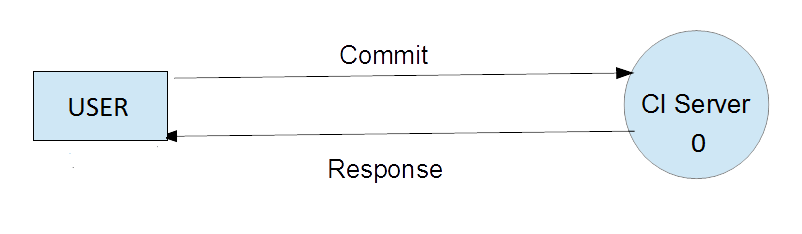
\epsfig{width=4in, file=dfd1.png}
\caption{Level 0 DFD}
\end{center}
\end{figure}

\subsection{Level 1 DFD}
The level 1 DFD gives a basic structure of the project indicating the five modules needed to execute the project.
\begin{figure}[h]
\begin{center}
\hspace{1 in}
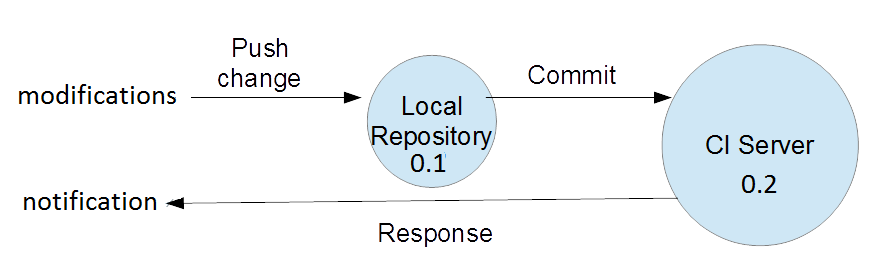
\epsfig{width=4in, file=dfd2.png}
\caption{Level 1.1 DFD}
\end{center}
\vspace{-1.5 in}
\end{figure}

%\begin{figure}[h]
%\begin{center}
%\epsfig{width=5in, file=dfd1_2.jpg}
%\caption{Level 1.1 DFD}
%\end{center}
%\end{figure}

\pagebreak
\subsection{Level 2 DFD}
The level 2 DFD gives a much more advanced idea about the execution. Each of these sections perform unique functions and these are combined together to yield the final product.
\begin{figure}[h]
\begin{center}
\vspace{0.5 in}
\hspace{.0 in}
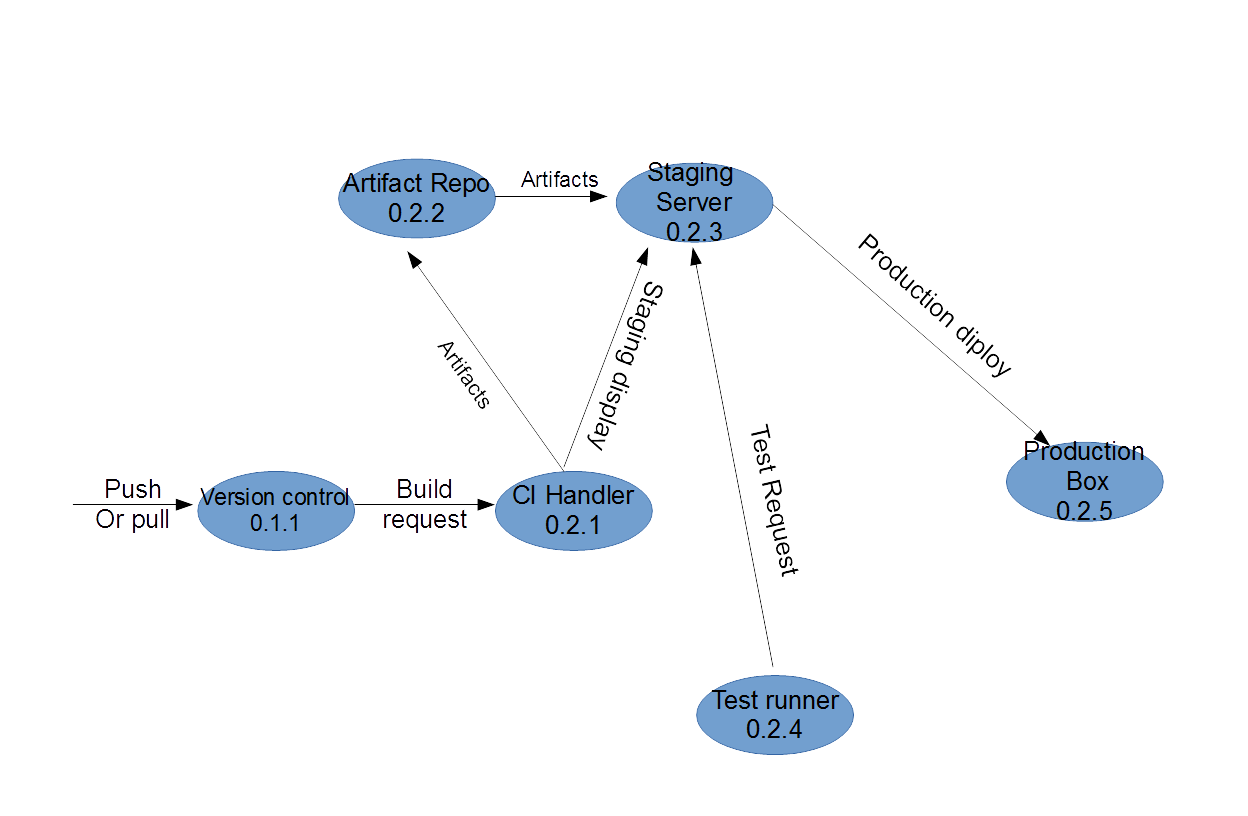
\epsfig{width=6in, file=dfd3.png}
\caption{Level 2.1.1 DFD}
\end{center}

\end{figure}
\pagebreak

\section{Flow Diagram}
\begin{figure}[h]
\begin{center}

\hspace{.0 in}
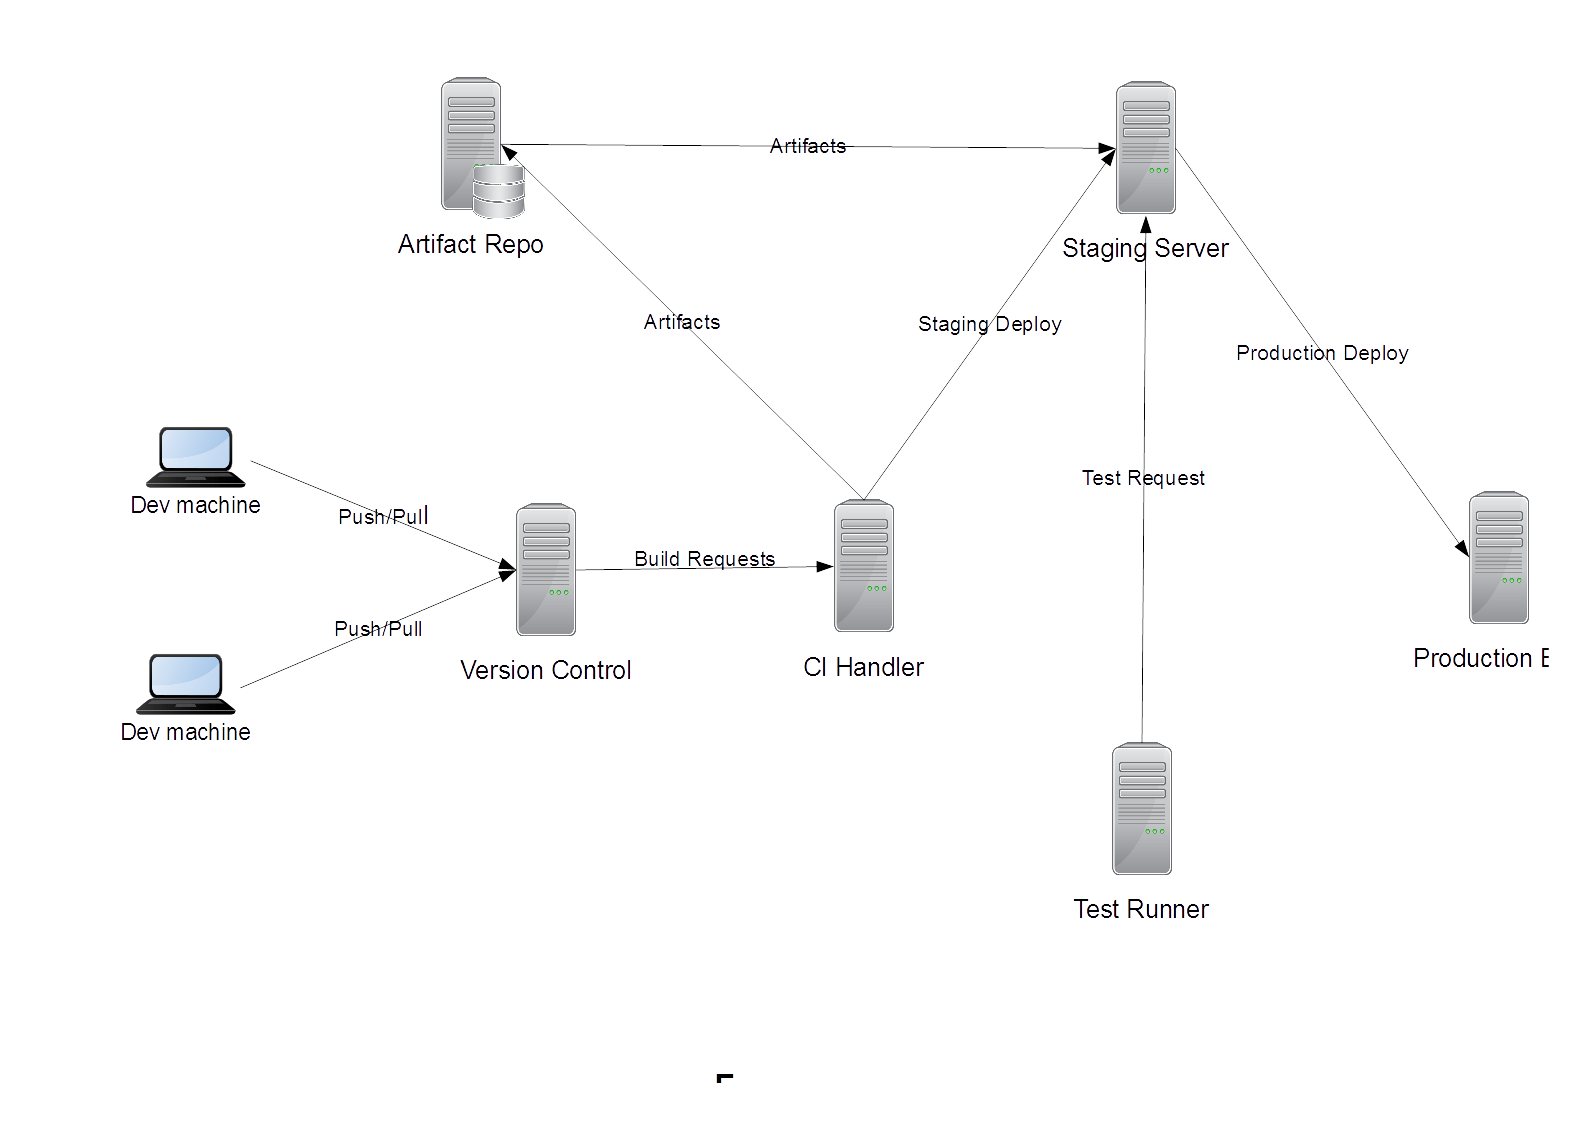
\epsfig{width=6in, file=flow1.png}
\caption{Flow diagram}
\end{center}

\end{figure}
\pagebreak
\section{C.I Pipeline Diagram}
\begin{figure}[h]
\begin{center}

\hspace{.0 in}
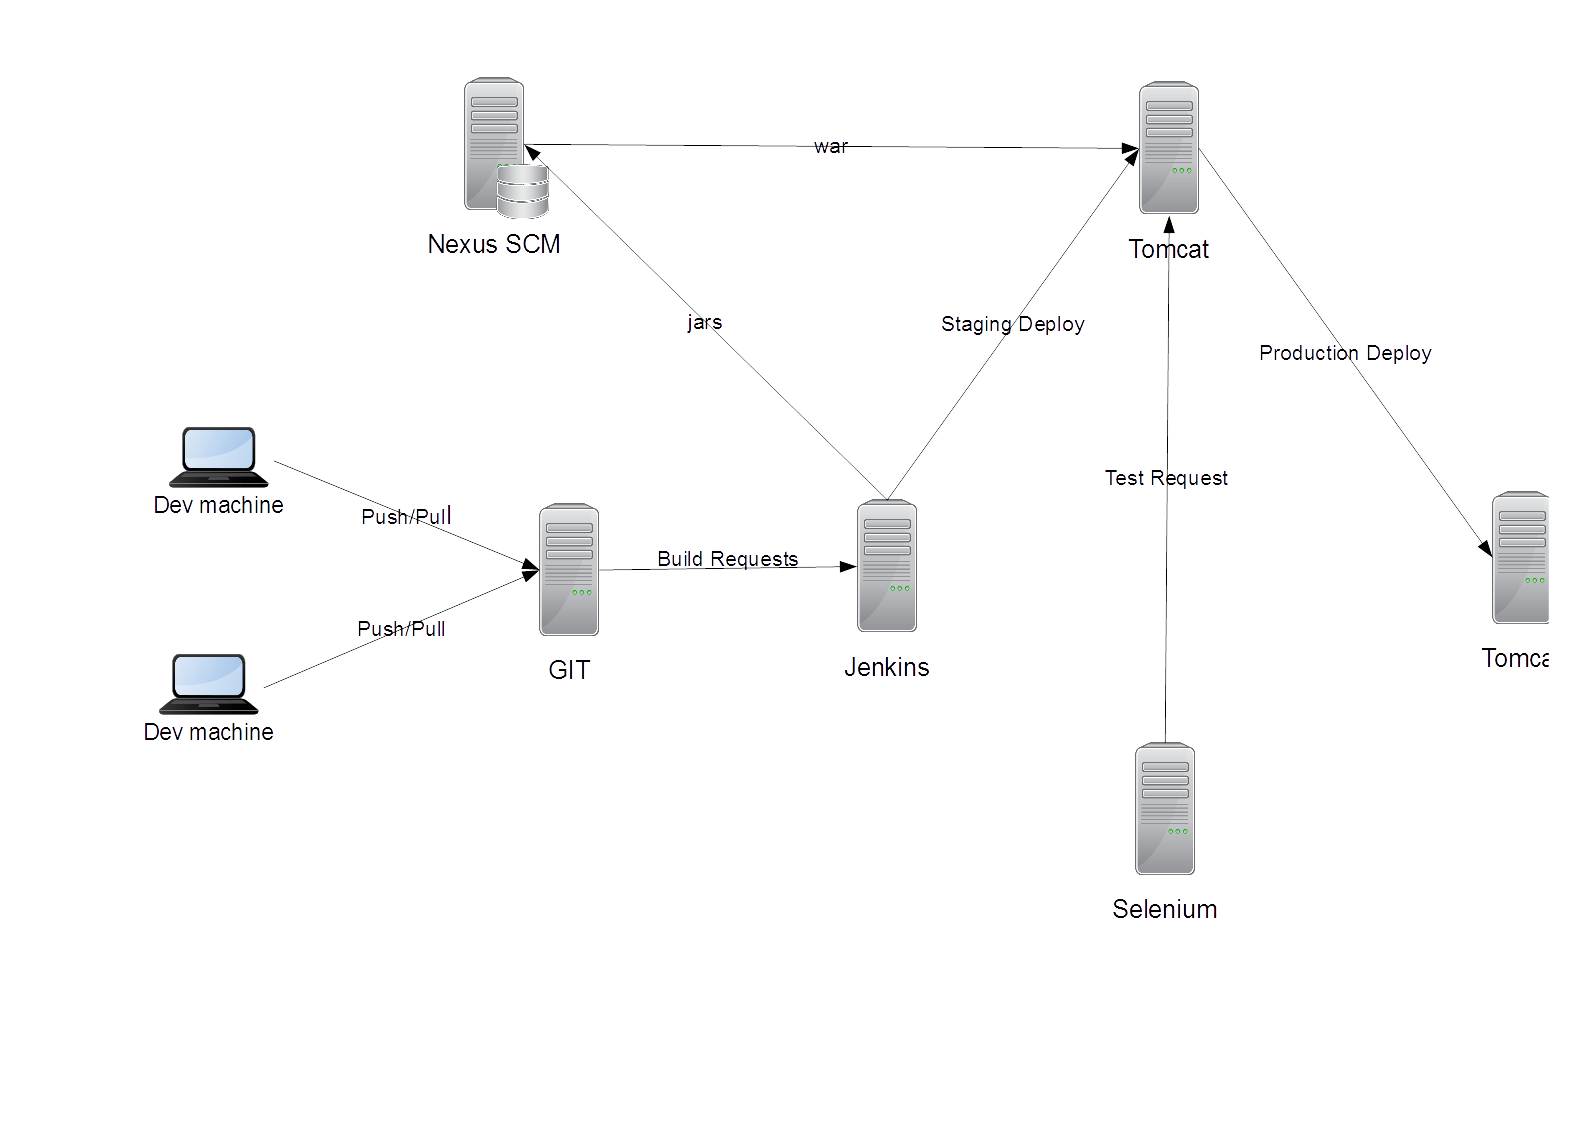
\epsfig{width=6in, file=pipeline.png}
\caption{C.I Pipeline}
\end{center}

\end{figure}
\pagebreak
\section{Sequence Diagram}
\par A Sequence diagram is an interaction diagram that shows how processes operate with
one another and in what order. It is a construct of a Message Sequence Chart. A sequence
diagram shows object interactions arranged in time sequence. It depicts the objects and classes
involved in the scenario and the sequence of messages exchanged between the objects needed
to carry out the functionality of the scenario.
\begin{figure}[h]
\begin{center}

\hspace{.0 in}
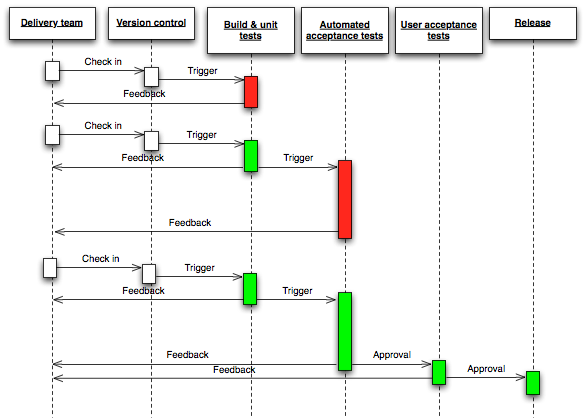
\epsfig{width=6in, file=sequence.png}
\caption{sequence}
\end{center}

\end{figure}

\chapter{METHODOLOGIES}
The product is completely been developed in Java environment in Windows platform. This chapter may explain our implementation details.

 \section{Languages And platforms Used}
The product is developing in Java as well as C++ environment. We are looking forward on Netbeans IDE 7.1 for networking and web page development. For interface we use swing and awt packages in Java8.0. The development will be carried out in LINUX platform and since we are depending only on Open Source softwares we may claim that we are technically feasible. The reason for selecting C++ as the language is been listed below.
	C++ is a powerful and flexible Open Source language.We use a library called
	\textbf{FANN}(Fast Artificial Neural Networks) to implement our neural network. 
Reason for using Java for developing the interface is given below.
Java is developed in the name of Green project, its Write Once Read Anywhere (WORA) feature makes it a powerful language packed with cross-platform dependence. Closely linked with the Object Oriented concept but not completely Object Oriented Language due to its Interface libraries, this language offers more security than any other languages do. It is the same platform independence feature of JAVA that tempts programmers and developers to build the networking application interfaces in J2EE environment.

\chapter{CONCLUSION}
Optical Character Recognition has it own significance nowadays. It has wide range of applications in the domain of postal automation, automatic number plate recognition,
preservation of handwritten historical documents,bank check processing,reading aid for the blind people
etc. Handwritten character recognition is traditionally divided into on-line and online recognition.We
are doing an on-line HCR system. 
\par  Even though HCR systems are well advanced in foreign language
scripts like Chinese and Japanese, only few works exist in Indian scripts especially in the South Indian
scripts. This is mainly due to its large character set, high degree of similarity between these characters
and the presence of compound characters in these scripts. Also, variations in the writing styles of different
people make the recognition process more difficult. Among the Indian languages, most of the work has
been reported in Devanagari and Bangla. The research on South Indian scripts namely Malayalam,
Tamil, Telugu and Kannada have gained much popularity recently as many agencies like the Ministry
of Communications and Information Technology and Government of India are providing aid and financial
support for many of these projects.


\renewcommand{\bibname}{Chapter 7\\\uppercase{REFERENCES}}
\begin{thebibliography}{999}
\addcontentsline{toc}{chapter}{8\hspace{0.1in} REFERENCES}

\bibitem{r1} 
Yalniz, I.Z.; Manmatha. R,
\quotes{A Fast Alignment
Scheme for Automatic OCR Evaluation of Books}
International Conference Document Analysis and
Recognition (ICDAR), 2011.

\bibitem{r2}  Jeff Heaton, \quotes{Introduction to neural networks in
Java, Heaton Research Inc., 2005,0-9773206-0-X.
[10]. Raman Maini and himanshuAggarwal, A
comprehensive review of image enhancement
techniques}, Journal of computing, volume 2, issue
3, 2010, ISSN 2151-9617.

\bibitem{r3} Brijmohan Singh, Mridula, Vivek Chand, Ankush
Mittal and D.Ghosh, \quotes{A comparative study of
different approaches of noise removal for document
images}, International conference on soft
computing for problem solving, volume 130/2102,
p 847-854, 2011.

\bibitem{r4}  ErginaKavallieratou and FotisDaskas,\quotes{Text line
detection and segmentation Uneven skew angles
and kill-and-dale writing}, Journal of Universal
computer science, Vol 17, p 16-29, 2010.

\bibitem{r5} Vatsal H. Shah\quotes{Machine Learning Techniques for Stock Prediction} 
\bibitem{r6} Robert Burbidge, Bernard Buxton, \quotes{An Introduction to Support Vector Machines for Data
Mining}
\textit{Computer Science Dept., UCL, Gower Street, WC1E 6BT, UK}

\bibitem{r7}C N Aganthopolous, \quotes {A License Plate Recognition
algorithm for Intelligent Transportation System
applications}. University of the Aegean and
National Technical University of Athens, p 377-
392, 2006.




\end{thebibliography}
\end{document}